\documentclass[border=10pt]{standalone}
\usepackage{tikz}\usepackage{amsmath}\usetikzlibrary{arrows.meta}
\begin{document}
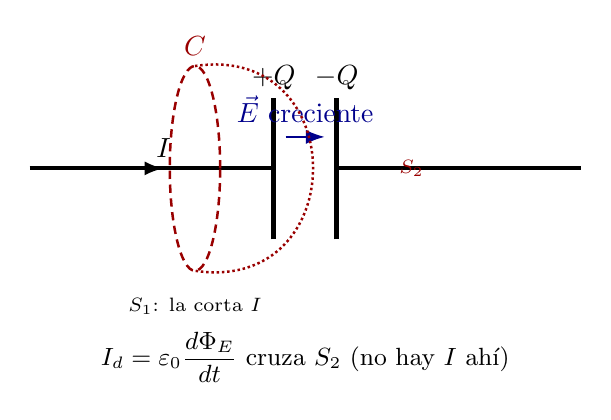
\begin{tikzpicture}[line width=0.9pt,>={Latex[length=2.4mm]}]
  % cable y condensador
  \draw[line width=1.4pt] (-3.5,0)--(-0.4,0);
  \draw[->,line width=1.1pt] (-2.6,0)--(-1.8,0) node[above]{$I$};
  \draw[line width=1.6pt] (-0.4,-0.9)--(-0.4,0.9); % placa izq
  \draw[line width=1.6pt] (0.4,-0.9)--(0.4,0.9);   % placa der
  \node at (-0.4,1.15){$+Q$}; \node at (0.4,1.15){$-Q$};
  \draw[->,blue!55!black] (-0.25,0.4)--(0.25,0.4); \node[blue!55!black] at (0,0.75){$\vec E$ creciente};
  \draw[line width=1.4pt] (0.4,0)--(3.5,0);
  % lazo amperiano (perpendicular, visto de canto) en el cable izq
  \draw[densely dashed,red!60!black] (-1.4,0) ellipse (0.32 and 1.3);
  \node[red!60!black] at (-1.4,1.55){$C$};
  % superficie 1 (plana, atravesada por I)
  \node at (-1.4,-1.75){\scriptsize $S_1$: la corta $I$};
  % superficie 2 (abombada hasta el hueco)
  \draw[densely dotted,red!60!black] (-1.4,1.3) .. controls (0.6,1.6) and (0.6,-1.6) .. (-1.4,-1.3);
  \node[red!60!black] at (1.35,0){\scriptsize $S_2$};
  \node at (0,-2.4){\small $\displaystyle I_d=\varepsilon_0\frac{d\Phi_E}{dt}$ cruza $S_2$ (no hay $I$ ahí)};
\end{tikzpicture}
\end{document}
